\chapter{Theoretische Grundlagen}\label{chapter:theorie}
%NOTES:
%-> verteilte systeme zeug
 %   -> sync and async data exchange
  %  -> verschlüsselung
   % -> Authentifizierung
 %   -> Business Data Objects (BDO)
%    -> 
%websockets
%opcua
%knoten und kanten
%datenbanken
%was ist eine db?
%-> normalformen
%-> referenzielle integrität
%-> sql
%webdevelopment
%-> js frameworks
%-> vue
%-> JSON
%-> XML
%-> REST
%interfaces
%->general
%->impl. in JS
%->impl. in C++
%\section{SCADA}
%\section{Verteilte Systeme}
%\subsection{Synchrones Datenmodell}
%\subsection{Asynchrones Datenmodell}
% \section{Security}\label{sec:security}
% \subsection{Authentifizierung}
% \subsection{Verschlüsselung}
\section{Websocket}
%Protokoll WS bzw WSS Präfix
Websockets bieten die Möglichkeit Nachrichten zwischen einem Server und einer Webanwendung asynchron auszutauschen.
Jede Websocket Verbindung startet zu Beginn als \ac{http} Verbindung. 
Der Client sendet einen \ac{http} Request vom Typ \emph{GET},
mit den Attributen \emph{Connection: Upgrade} und \emph{Upgrade: websocket} im Header, an den \ac{http} Server.
Unterstützt der \ac{http} Server das Websocket Protokoll, 
bestätigt er die Anfrage mit einem \emph{HTTP/1.1 101 Switching Protocols} Response.
Anschließend bauen die Teilnehmer eine \ac{tcp} Verbindung auf, die so lange bestehen bleibt, bis einer der Teilnehmer die Verbindung aktiv beendet 
oder ein Teilnehmer nicht mehr erreichbar ist.
Die ausgetauschten Daten können Strings oder binäre Daten sein. Beides wird vom Websocket Protokoll unterstützt.
Das Protokoll definiert allerdings keine Semantik der übertragenen Daten, 
weshalb immer ein Subprotokoll nötig ist, um damit produktiv zu arbeiten.
Wie auch eine \ac{http} Verbindung, kann eine Websocket Verbindung verschlüsselt werden. Dies erkennt man am Protokollpräfix des \ac{url}.
Bei einer unverschlüsselten Verbindung lautet der Präfix \eigenName{ws://} und bei einer verschlüsselten Verbindung \eigenName{wss://}.

\section{Datenbanken}
Der Zweck eines Datenbanksystems ist es, Daten persistent zu speichern und zur Verfügung zu stellen.
Ein Datenbanksystem setzt sich aus einer Datenbasis, sowie einem \ac{dbms} zusammen.
Dabei stellt die Datenbasis den Speicher der Datenbank dar und das \ac{dbms} 
das Programm durch das der Zugriff auf die Datenbasis ermöglicht wird.
Das \ac{dbms} ist notwendig, um konkurrierende Zugriffe von mehreren Nutzer auf die selbe Datenbasis zu verwalten \citep{Schubert:2007:3}. 
Meistens bietet das \ac{dbms} als Interface eine Netzwerkschnittstelle an (Server-Client Architektur), es gibt allerdings auch Datenbanken deren \ac{dbms} Teil der Applikation werden (z.B. SQLite).

\subsection{Relationale Datenbank}\label{subsec:relDB}
Im Falle einer relationalen Datenbank werden Daten in Form von Relationen abgespeichert.
Tabellen sind eine Darstellung von Relationen.\\
Jede Relation hat Attribute mit einem in der Relation einzigartigem Attributnamen.
Die Domäne eines Attributs ist die Menge aller Werte, die ein Attribut annehmen kann.
Ist der Wert eines Attributs unbekannt oder noch nicht bestimmt, ist der Wert des Attributs \eigenName{NULL} \citep{Studer:2016:2}.
Werden Daten nun in einer Datenbank gespeichert, wird ein Wertetupel in eine Relation eingefügt.
Die Relationen sind nur das strukturelle theoretische Konzept, das sich hinter einer relationalen Datenbank verbirgt.
Anfangs dieses Abschnitts wurde gesagt, dass Relationen in Form einer Tabelle darstellbar sind.
Wenn Relationen nun zu ihrer Definition Wertetabellen zu Grunde liegen, 
ist es möglich zur Vereinfachung statt von Relationen von Tabellen zu sprechen.
Das \ac{dbms} stellt eine Schnittstelle bereit um dem Nutzer die Daten zugänglich zu machen (\ac{crud} Operationen).
Die Schnittstelle unterstützt meist die Sprache \ac{sql}. Diese Sprache ist in Abschnitt \ref{subsec:sql} genauer beschrieben.
Relationen können nicht nur als Tabelle ausgegeben werden, es ist auch möglich sie zu verknüpfen.
Wenn keine Regel angegeben wird wie zwei Relationen verknüpft werden sollen, wird das informatische Kreuzprodukt gebildet.
Das bedeutet, dass jedes Wertetuple aus Relation A, mit jedem Wertetupel aus Relation B verknüft wird. 
Dadurch entsteht eine neue Relation.
In einer Datenbank existieren immer Schlüssel (Keys) innerhalb einer Tabelle.
Dabei gibt es drei Typen:
\begin{itemize}
  \item Primary-Key (Primärschlüssel)
  \item Unique-Key
  \item Foreign-Key (Fremdschlüssel)
\end{itemize}
Der Primary-Key muss als einziger Schlüssel zwingend vorhanden sein. Er bestimmt nach was das \ac{dbms} die Datensätze ablegt.
Deshalb muss der Wert des Attributes das den Primary-Key bildet, innerhalb einer Tabelle einzigartig sein.
Das heißt, es darf maximal ein Wertetupel mit dem selben Wert des Primärschlüssels, innerhalb einer Relation, existieren.
Der Primärschlüssel darf auch nicht \eigenName{NULL} sein.
Ein Unique-Key stellt einen zusätzlichen Schlüssel dar, über die jeder Eintrag in einer Tabelle eindeutig identifizierbar ist.
Wie auch der Primärschlüssel, darf dieser Schlüssel nicht \eigenName{NULL} sein.
Er ist in jeder Tabelle nur optional vorhanden. Es ist allerdings auch möglich dass mehrere Unique-Keys existieren.
Der Foreign-Key (Fremdschlüssel) ist ein Schlüssel, der nur in einem relationalen \ac{dbms} unterstützt wird.
Er ermöglicht es, einen Verweis auf eine andere Tabelle zu definieren.
Zur Veranschaulichung sei folgendes Beispiel einer relationalen Datenstruktur,
auf einem \ac{sql} Server, gegeben.

\begin{figure}[ht]
  \centering
  \begin{subfigure}[h]{\textwidth}
    \centering
    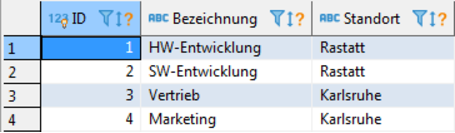
\includegraphics[width=0.517045455\textwidth]{content/hauptteil/theoretischeGrundlagen/rec/exampleSQLAbteilung.pdf}
    \caption{Tabelle \eigenName{Abteilung}}
    \label{fig:exampleSQLStructure:abteilung}
    \hspace{50.00mm}
  \end{subfigure}
  \begin{subfigure}[h]{\textwidth}
      \centering
      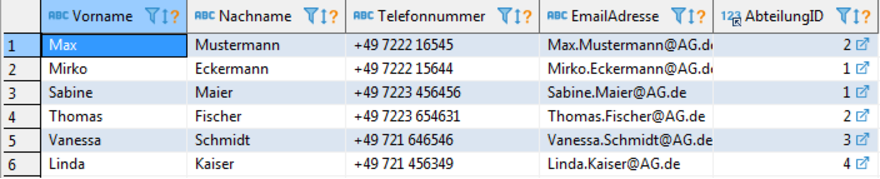
\includegraphics[width=\textwidth]{content/hauptteil/theoretischeGrundlagen/rec/exampleSQLMitarbeiterdaten.pdf}
      \caption{Tabelle \eigenName{Mitarbeiter}}
      \label{fig:exampleSQLStructure:mitarbeiter}
      \hspace{50.00mm}
  \end{subfigure}
  \begin{subfigure}[h]{\textwidth}
      \centering
      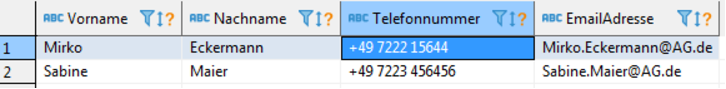
\includegraphics[width=0.825284091\textwidth]{content/hauptteil/theoretischeGrundlagen/rec/exampleSQLErgebnis.pdf}
      \caption{Ergebnis des Querys aus \refFig{fig:exampleSQLQuery}}
      \label{fig:exampleSQLStructure:result}
  \end{subfigure}
  \caption[Beispiel Datenstruktur mit Ergebnis von einem \eigenName{Join} Query]{Eigene Beispiel Datenstruktur als Tabellen mit Ergebnis des Querys aus \refFig{fig:exampleSQLQuery}}
  \label{fig:exampleSQLStructure}
\end{figure}
Wie in der Abbildung \ref{fig:exampleSQLStructure} zu sehen ist, besteht die Datenbank aus zwei Tabellen.
Die erste Tabelle hat die Bezeichnung \eigenName{Abteilung} (\refFig{fig:exampleSQLStructure:abteilung}) mit den Spalten \eigenName{ID}, \eigenName{Bezeichnung} sowie \eigenName{Standort}.
Die Spalte \eigenName{ID} ist als Primary-Key deklariert.
Die zweite Tabelle \eigenName{Mitarbeiter} (\refFig{fig:exampleSQLStructure:mitarbeiter}) enthält die Spalten 
\eigenName{Personalnummer}, \eigenName{Vorname}, \eigenName{Nachname}, \eigenName{Telefonnummer}, \eigenName{EmailAdresse} und \eigenName{AbteilungID}.
In dieser Tabelle ist die Personalnummer der Primärschlüssel.
Um eine Verknüpfung der Spalte \eigenName{AbteilungID} der Tabelle \eigenName{Mitarbeiter} zu der Tabelle \eigenName{Abteilung} herzustellen, 
wird ein Fremdschlüssel definiert, der von der Spalte \eigenName{AbteilungID} der Tabelle \eigenName{Mitarbeiter} auf die Tabelle \eigenName{Abteilung}, 
unter Benutzung deren Primärschlüssels, verweist.
Die Definition eines Fremdschlüssels ist nicht zwingend notwendig, um die Verknüfung der zwei Relationen nach dieser Semantik zu ermöglichen.
Es ermöglicht aber die selbstständige Erhaltung der referenziellen In­te­g­ri­tät durch das \ac{dbms}. 
Dabei hat man bei der Erstellung des Fremdschlüssels die Wahl, was beim Löschen oder beim Ändern eines referenzierten Datensatzes geschehen soll.
Der gängigste Umgang damit ist, dass man entweder das Löschen verbietet (\emph{on delete restrict}),
oder das beim Löschen des referenzierten Datensatzes auch der referenzierenden Datensatz gelöscht wird (\emph{on delete cascade}).
Bei beiden Verfahren bleibt die referenzielle In­te­g­ri­tät erhalten.
Das heißt es gibt nach dem Löschen keine Referenzen, die nicht aufgelöst werden können.

\subsection{\acs{sql}}\label{subsec:sql}
\acs{sql} ist eine Abkürzung für \acl{sql}. Dabei handelt es sich um eine herstellerunabhängige Sprache, 
welche das Erzeugen und Verwalten von Datenstrukturen ermöglicht. 
Außerdem ermöglicht sie das Abfragen, Einfügen, Verändern, sowie Verknüpfen von Datensätzen.
Dabei unterscheidet sich \ac{sql} sehr von anderen Programmiersprachen.
So besteht der Ansatz bei \ac{sql} eher darin zu definieren, was man als Ergebnis möchte, 
sich aber um die konkrete Implementierung der Operation keinerlei Gedanken zu machen braucht.
Um dies zu demonstrieren, ist das folgende Beispiel, auf Basis der Beispieldatenbank in Abbildung \ref{fig:exampleSQLStructure}, gegeben.
Nun möchte man alle Telefonnummern, Namen und E-Mail Adressen einer Abteilung haben, welche den Namen \emph{HW-Entwicklung} trägt.
Dazu ist es notwendig die Datensätze der Mitarbeitertabelle mit den Datensätzen der Abteilungstabelle, 
entsprechend des Fremdschlüssels in der Mitarbeiter Tabelle, zu kombinieren und alle Datensätze der so entstandenen Tabelle auszugeben, 
welche die Abteilungsbezeichnung \emph{HW-Entwicklung} tragen. 
Die Query für diese Operation ist in Abbildung \ref{fig:exampleSQLQuery} abgebildet.
\begin{figure}[hbt]
  %\centering
  %\inputsql{content/hauptteil/theoretischeGrundlagen/rec/sqlQuery.sql}
  \inputminted{sql}{content/hauptteil/theoretischeGrundlagen/rec/sqlQuery.sql}
  \caption{Eigenes Beispiel SQL Query - Select mit Join}
  \label{fig:exampleSQLQuery}
\end{figure}
Die Antwort des Servers ist in \refFig{fig:exampleSQLStructure:result} zu sehen.
Bei \refFig{fig:exampleSQLStructure:abteilung} und \refFig{fig:exampleSQLStructure:mitarbeiter} sieht man die Datensätze der beiden Quelltabellen des Querys.
Wahrscheinlich würde man diesen einfachen Datenbank Join, in C/C++, mit den Daten in Structures gespeichert, mittels verschachtelter For-Schleifen implementieren. 
Das Problem bei dieser Implementierung ist, dass man durch jedes Element iterieren muss.
Das \ac{dbms} hat zur Lösung dieses Problems bessere Algorithmen hinterlegt (Stichwort: binärer Suchbaum, Hash-Maps\dots).

\subsection{Stored Procedures}\label{subsec:storedProc}
Ein \ac{sql} Server unterstützt nicht nur das Manipulieren und Ausgeben von Daten mit \ac{sql}, sondern auch das Speichern von Funktionen und Prozeduren.
Diese Prozeduren und Funktionen sind auch in \ac{sql} geschrieben.
Sie ermöglichen dem Entwickler das Auslagern komplexer \ac{sql} Querys.
Der wesentliche Unterschied zwischen einer Prozedur und einer Funktion besteht darin, dass eine Funktion einen Rückgabewert haben kann, eine Prozedur dagegen nicht.
Das Fehlen eines Rückgabewerts einer Prozedur stellt aber, entgegen der allgemeinen Erwartung, keine Einschränkung dar. 
Prozeduren und Funktionen akzeptieren auch sessionbezogene globale Variablen als \emph{OUT} Argument. 
Desweiteren haben Prozeduren entgegen Funktionen die Möglichkeit, \ac{sql} Querys zur Laufzeit zusammenzusetzen und auszuführen.
Funktionen können, in \ac{sql} Querys benutzt werden, Prozeduren nicht.
Prozeduren werden durch ein \emph{CALL} Befehl aufgerufen.

\section{OPC UA}
\ac{opcua} ist ein Thema, das immer wieder mit Industrie 4.0 in Verbindung gebracht wird.
\citet{opcua:2018} fasst \acs{opcua} in wenigen  Worten zusammen:\\
\eigenNameUmbr{OPC UA (Open Platform Communications Unified Architecture) ist eine Sammlung von Standards 
für die Kommunikation und den Datenaustausch im Umfeld der Industrieautomation. 
Mithilfe von OPC UA werden sowohl der Transport von Machine-to-Machine-Daten 
als auch Schnittstellen und die Semantik von Daten beschrieben. 
Die komplette Architektur ist serviceorientiert aufgebaut.}\\
Eine der großen Herausforderungen der Industrie 4.0 besteht in der Vernetzung aller Geräte in einer Fabrik.
Dies ist nur durch die Verwendung eines offenen (herstellerunabhängigen) Standards möglich.
Ein solcher Standard ist \ac{opcua}. 
Er definiert nicht nur wie Daten ausgetauscht werden, 
sondern auch wie die Daten zu interpretieren sind (Semantik).
Dabei bedient sich ein \ac{opcua} Server einem eingebauten Informationsmodell. 
Dies kann man sich wie Klassen und Objekte in der objektorientierten Programmierung vorstellen.
Als Beispiel bietet Hersteller A eine Pumpe am Markt an. 
Diese Pumpe besitzt eine \ac{opcua} Schnittstelle (Server).
Dieser Server hat ein Pumpenobjekt mit der Bezeichung \eigenName{pumpe\_xyz\_A}, das eine Menge an Attributen besitzt die man lesen, schreiben, oder lesen und schreiben kann.
Jedes Attribut hat einen eindeutigen Datentyp. 
Das Attribut \emph{Seriennummer} besitzt zum Beispiel den primitiven Typ \emph{String}.
Ein \ac{opcua} Server unterstützt aber nicht nur primitive Datetypen, 
sondern auch Objekte wie das Pumpenobjekt \eigenName{pumpe\_xyz\_A} des Herstellers A.
Nun möchte man diese Pumpe des Herstellers A durch ein \ac{plc} des Herstellers B auslesen beziehungsweise steuern.
Bei einer propriotären Schnittstelle, würde dies zu Problemen führen da dem Hersteller B das Informationsmodell der Pumpe nicht bekannt ist. 
Hersteller A müsste in diesem Fall Dokumente liefern, mit denen Hersteller B die Pumpe ansteuern könnte. Diese wäre zum Beispiel eine \ac{edd} Datei.
Der Hersteller wäre also gezwungen, für jeden größeren \ac{plc} Hersteller, verschiedene Dokumente zur Verfügung zu stellen.

\ac{opcua} geht an dieser Stelle einen anderen Weg. 
Der \ac{opcua} Standard stellt eine Menge an \ac{opcua} Klassen zur Verfügung, 
von denen die Hersteller nun ihre eigenen Klassen ableiten können.
Eine solche Klasse gibt es auch für eine Pumpe. Diese Klasse besitzt nun die minimalen Attribute einer Pumpe.
Hersteller A leitet nun ihre Pumpenklasse (\eigenName{pumpe\_xyz\_A}) von dieser Pumpenklasse ab und erweitert die Klasse um ihre eigenen zusätzlichen Attribute.
Wenn jetzt Hersteller B die Pumpe mit ihrem \ac{plc} ansprechen möchte, gibt es zwei Möglichkeiten.
Es ist bekannt, dass die Pumpenklasse \eigenName{pumpe\_xyz\_A} von der allgemeinen Pumpenklasse des Standards abgeleitet wurde.
Damit ist es möglich, zumindest die minimalen Funktionen der Pumpe, anzusprechen. 
Möchte man sich nicht darauf beschränken, sondern den vollen Funktionsumfang nutzen, den die Pumpe bietet, 
so kann der \ac{plc} sich bei dem \ac{opcua} Server nach deren Informationsmodell für die Pumpe erkundigen.
Die Attribute sind damit nicht nur in ihrem Typ bekannt, sondern auch in ihrer Bedeutung (Semantik).
Als Transportprotokoll benutzt \ac{opcua} das \ac{ip}. 
Damit ist eine horizontale sowie vertikale Vernetzung innerhalb der Automatisierungspyramide möglich \citep{opcua:2018}.
\ac{opcua} untersützt dabei ein Konzept bei dem Daten angefragt werden (zyklisches lesen), sowie ein Publish/Subscribe Konzept, 
bei dem man sich Datenknoten abonnieren kann und fortan von dem Server über Änderungen informiert wird \citep{opcua:2018}.

\section{Echtzeit}
Laut \citet{Scholz:2005} ist Echtzeit wie folgt definiert:\\
\eigenName{Unter Echtzeit versteht man den Betrieb
eines Rechensystems, bei dem Programme zur Verarbeitung
anfallender Daten ständig betriebsbereit sind, derart, dass die
Verarbeitungsergebnisse innerhalb einer vorgegebenen Zeitspanne
verfügbar sind. Die Daten können je nach Anwendungsfall nach
einer zeitlich zufälligen Verteilung oder zu vorherbestimmten
Zeitpunkten anfallen.}\\
Das bedeutet, dass ein System nur dann echtzeitfähig ist, wenn es die folgenden Bedingungen erfüllt:
\begin{itemize}
  \item Jede Komponente des Systems, die an dem Prozess beteiligt ist, muss selbst echtzeitfähig sein.
  \item Die Rechenzeit der verwendeten Algorithmen muss endlich sein und deren Maximum kalkulierbar.
  \item Die Transportprotokolle, die beteiligt sind dem Prozess Daten zuzuführen bzw. Daten zu entnehmen, müssen die Echtzeitfähigkeit unterstützen.
\end{itemize}
Wenn die obere Definition nun auf das Ethernet oder das \ac{tcp} Protokoll angewand wird, fällt schnell auf, 
dass diese beide normalerweise nicht echtzeitfähig sind.
Ethernet verhindert auf dem Bus (physikalischer Layer) keine Kollisionen sondern erkennt diese nur. 
Wenn eine Kollision erkannt wurde, 
wird das Senden auf dem Bus abgebrochen und nach einer zufälligen Zeit erneut versucht.
Dieses Verfahren nennt man \ac{CSMA/CD}. 
Den Buszugriff erhält immer der Teilnehmer der zuerst sendet. Wann ein anderer Teilnehmer dann den Buszugriff erhält ist Zufall.
Deshalb ist nicht garantiert, dass man innerhalb einer definierten Zeitspanne die Daten übertragen kann.
Man kann dieses Problem allerdings umgehen, indem man im physikalischen Layer bereits dafür sorgt, 
dass keine Datenkollision auftreten kann. Dies ist zum Beispiel durch den Einsatz von Switches möglich.
Diese trennen die einzelnen Sender voneinander, sodass innerhalb einer Kollisiondomäne sich immer nur ein Sender befindet. Damit ist es möglich Kollisionen gezielt zu verhindern.

Es muss an dieser Stelle angemerkt werden, dass man immernoch nicht vollständig echtzeitfähig Daten übertragen kann, 
da das Netzwerk auch auf die aufkommende Datenlast ausgelegt sein muss.
Dadurch ist es möglich mit Ethernet in einer kontrollierten Umgebung Daten in Echtzeit zu übertragen.
Ein weitverbreiteter Irrtum ist, dass Echtzeitfähigkeit bedeutet etwas müsse besonders schnell reagieren, 
es genügt dass die Reaktionszeit definiert und endlich ist.